\chapter{Anhang}\label{app:anhang}
\section{Steckbriefe der Personas}\label{persona}
Im Folgenden sind die Steckbriefe der Personas Thorsten und Mark zu sehen. Was für einen Zweck diese erfüllen, wird in Abschnitt \ref{inhaltliche_anforderungen} erklärt.

\begin{figure}[!htb]
\minipage{0.48\textwidth}
  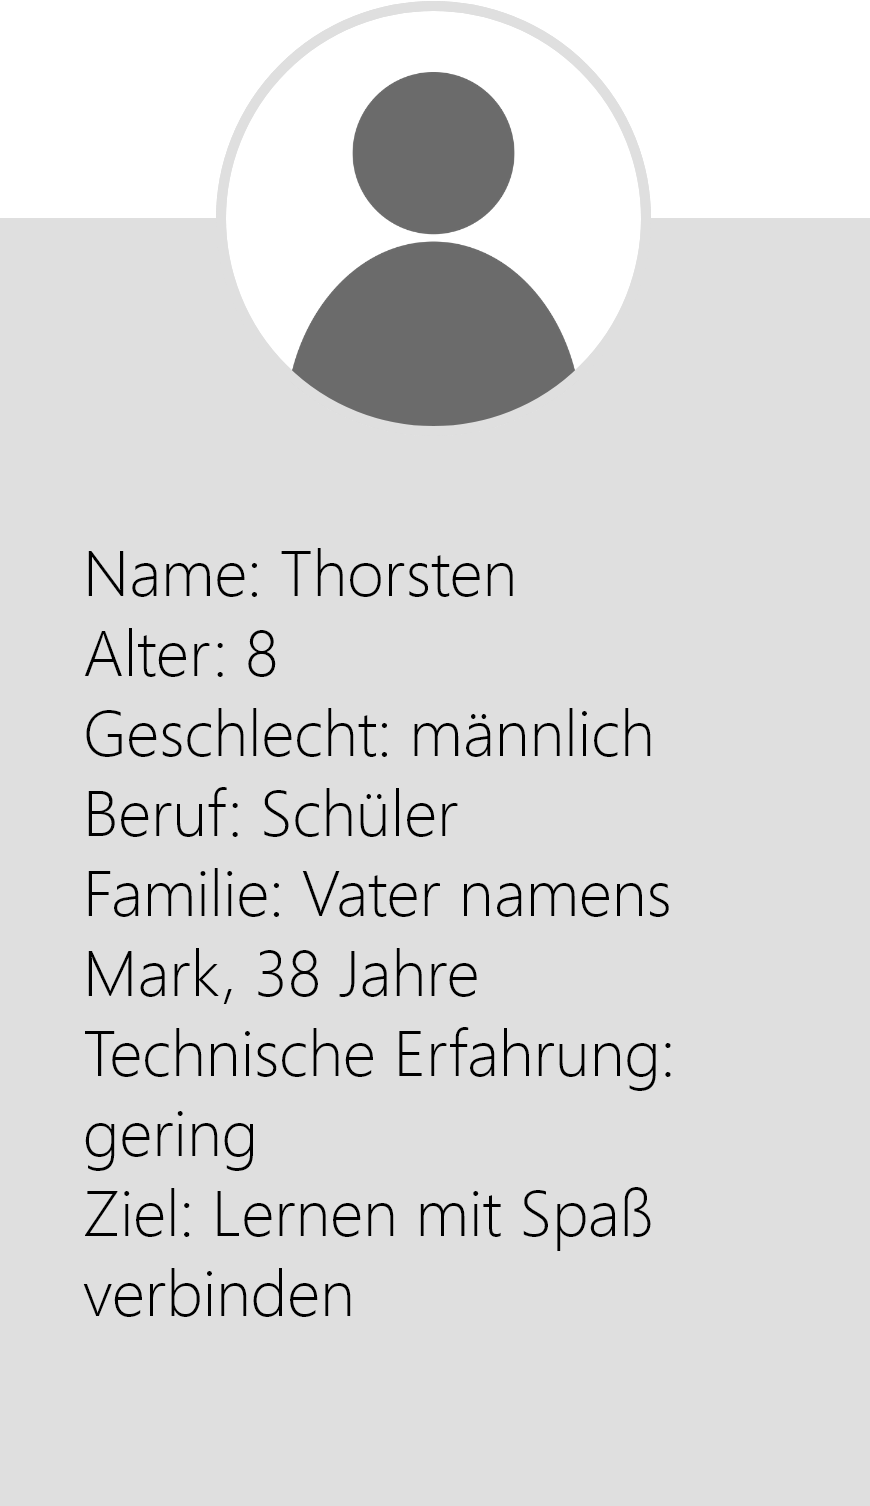
\includegraphics[width=\linewidth]{Persona_1.png}
  \caption{Steckbrief von Thorsten}\label{fig:persona_thorsten}
\endminipage\hfill
\minipage{0.48\textwidth}
  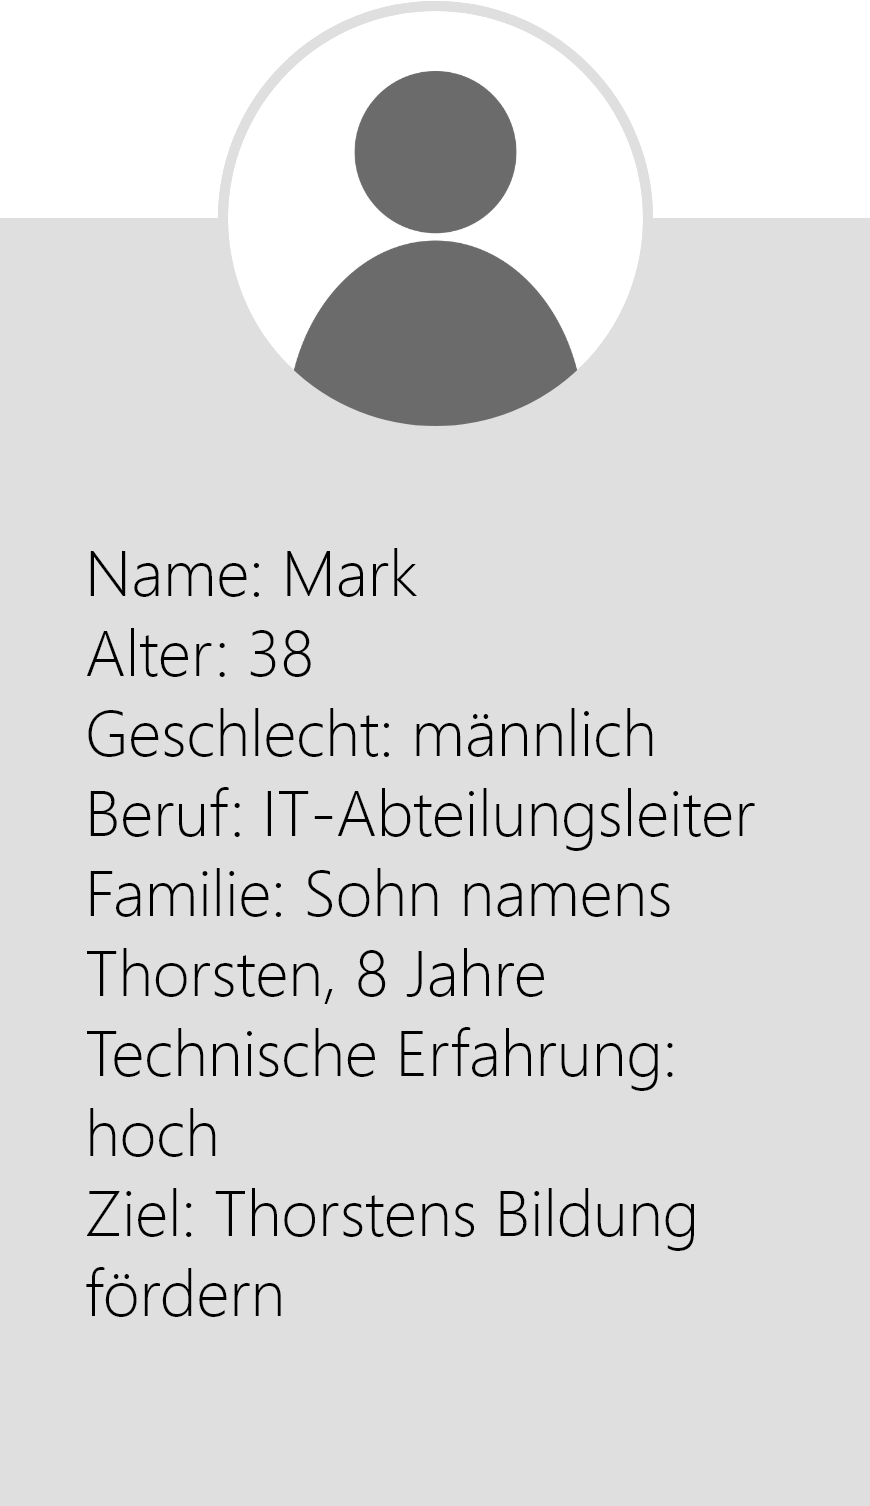
\includegraphics[width=\linewidth]{Persona_2.png}
  \caption{Steckbrief von Mark}\label{fig:persona_mark}
\endminipage\hfill
\end{figure}

\section{Meilensteinplan}\label{Meilensteinplan}

\textbf{Meilenstein 1 \textquote{Anforderungsanalyse} (ca. 2 Wochen):}
\begin{itemize}
\item Grafische Flowcharts (Navigation durch App) -> inhaltlicher Sinn der App
\item User Stories
\end{itemize}

\textbf{Meilenstein 2 \textquote{Recherche und Planung} (ca. 3 Wochen):}
\begin{itemize}
\item Evaluation und Festlegung der Techniken und Methoden (z.b. Datenbankanbindung, AR Funktionalität, Datenauswertung, ...)
\item grobe Architekturplanung
\end{itemize}

\textbf{Meilenstein 3 \textquote{Organisation} (ca. 2 Wochen):}
\begin{itemize}
\item Aufteilung der Zuständigkeiten (z.B. Aufteilung in Frontend/Backend)
\item Projektumgebung aufsetzen (Versionsverwaltung, Entwicklungsumgebung, Organisationstools, etc.)
\item Festlegung des Styleguides
\end{itemize}

\textbf{Meilenstein 4 \textquote{Entwurf} (ca. 3 Wochen):}
\begin{itemize}
\item Architekturplanung (Klassendiagramm, Datenbankmodell, etc.)
\item Entwurf von GUI-Mockups
\end{itemize}

\textbf{Meilenstein 5 \textquote{Implementierung}:}
\begin{itemize}
\item Erprobung der AR Technologie (3D Objekte finden und einfügen, Marker für Mustererkennung)
\item Initialapp generieren (Datenbankanbindung, Frontend, ...)
\item Implementierung der AR Funktionalität
\item Implementierung der In-App Navigation
\item Füllen der App mit Seiteninhalten
\item Inhalte für Quiz überlegen
\item ...
\end{itemize}

\section{Verwendete 3D Objekte}
Die für das Projekt verwendeten 3D Objekte werden im Folgenden mit ihrem zugehörigen Kontinent dargestellt. Diese entstammen verschiedenen Internetquellen, die in Abschnitt \ref{verwendung_3d_objekte} aufgeführt sind.

\begin{figure}[!htb]
\minipage{0.48\textwidth}
  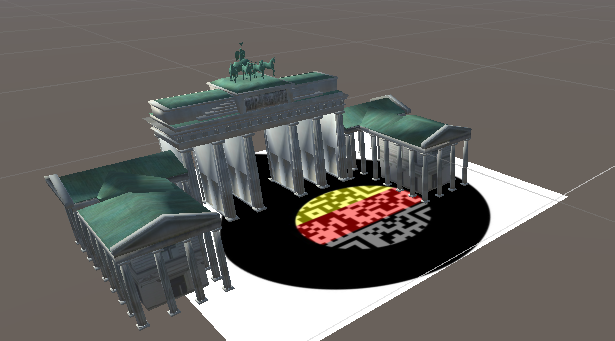
\includegraphics[width=\linewidth]{Deutschland.png}
  \caption{3D Objekt von Deutschland (Europa)}\label{fig:deutschland}
\endminipage\hfill
\minipage{0.48\textwidth}
  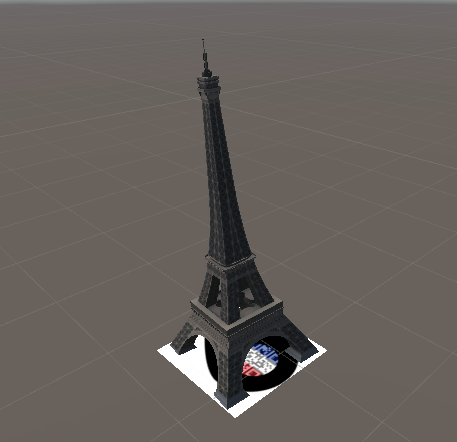
\includegraphics[width=\linewidth]{Frankreich.png}
  \caption{3D Objekt von Frankreich (Europa)}\label{fig:frankreich}
\endminipage\hfill
\end{figure}

\begin{figure}[!htb]
\minipage{0.48\textwidth}
  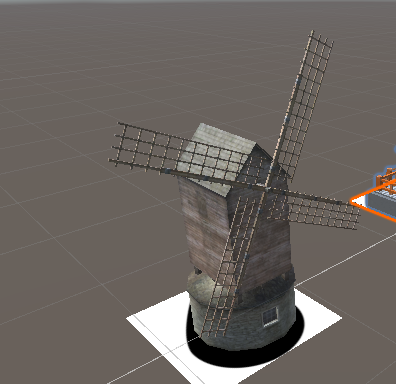
\includegraphics[width=\linewidth]{Niederlande.png}
  \caption{3D Objekt von den Niederlanden (Europa)}\label{fig:niederlande}
\endminipage\hfill
\minipage{0.48\textwidth}
  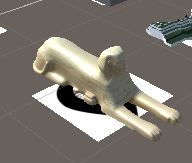
\includegraphics[width=\linewidth]{Aegypten.png}
  \caption{3D Objekt von Ägypten (Afrika)}\label{fig:aegypten}
\endminipage\hfill
\end{figure}

\begin{figure}[!htb]
\minipage{0.48\textwidth}
  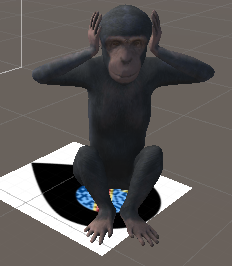
\includegraphics[width=\linewidth]{Kongo.png}
  \caption{3D Objekt vom Kongo (Afrika)}\label{fig:kongo}
\endminipage\hfill
\minipage{0.48\textwidth}
  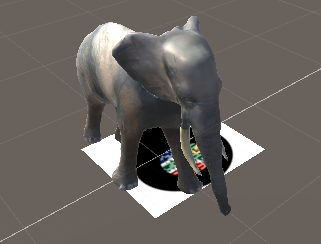
\includegraphics[width=\linewidth]{Suedafrika.png}
  \caption{3D Objekt von Südafrika (Afrika)}\label{fig:suedafrika}
\endminipage\hfill
\end{figure}

\begin{figure}[!htb]
\minipage{0.48\textwidth}
  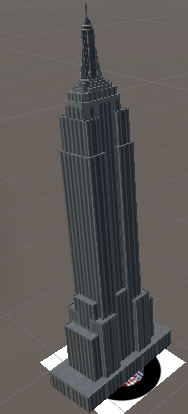
\includegraphics[width=\linewidth]{USA.png}
  \caption{3D Objekt von den USA (Nordamerika)}\label{fig:usa}
\endminipage\hfill
\minipage{0.48\textwidth}
  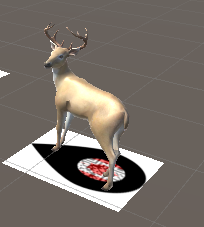
\includegraphics[width=\linewidth]{Kanada.png}
  \caption{3D Objekt von Kanada (Nordamerika)}\label{fig:kanada}
\endminipage\hfill
\end{figure}

\begin{figure}[!htb]
\minipage{0.48\textwidth}
  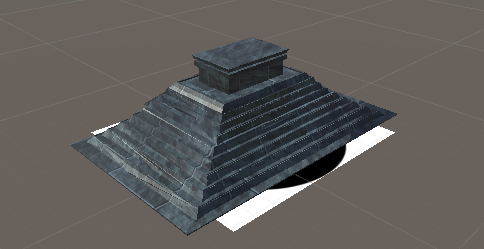
\includegraphics[width=\linewidth]{Mexiko.png}
  \caption{3D Objekt von Mexiko (Nordamerika)}\label{fig:mexiko}
\endminipage\hfill
\minipage{0.48\textwidth}
  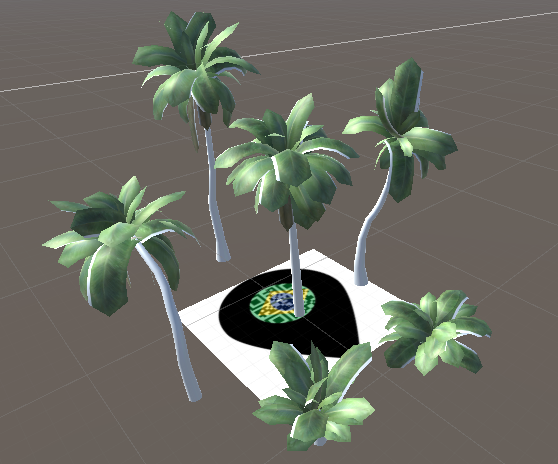
\includegraphics[width=\linewidth]{Brasilien.png}
  \caption{3D Objekt von Brasilien (Südamerika)}\label{fig:brasilien}
\endminipage\hfill
\end{figure}

\begin{figure}[!htb]
\minipage{0.48\textwidth}
  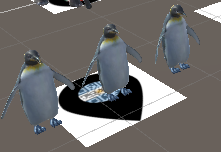
\includegraphics[width=\linewidth]{Argentinien.png}
  \caption{3D Objekt von Argentinien (Südamerika)}\label{fig:argentinien}
\endminipage\hfill
\minipage{0.48\textwidth}
  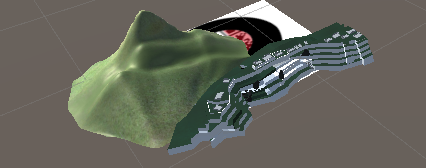
\includegraphics[width=\linewidth]{Peru.png}
  \caption{3D Objekt von Peru (Südamerika)}\label{fig:peru}
\endminipage\hfill
\end{figure}

\begin{figure}[!htb]
\minipage{0.48\textwidth}
  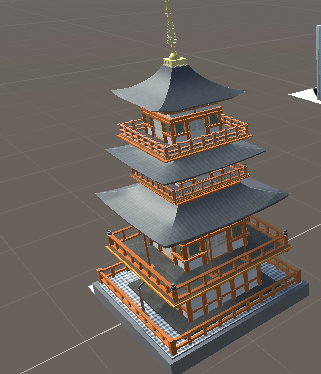
\includegraphics[width=\linewidth]{Japan.png}
  \caption{3D Objekt von Japan (Asien)}\label{fig:japan}
\endminipage\hfill
\minipage{0.48\textwidth}
  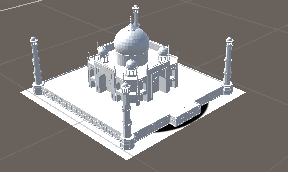
\includegraphics[width=\linewidth]{Indien.png}
  \caption{3D Objekt von Indien (Asien)}\label{fig:indien}
\endminipage\hfill
\end{figure}

\begin{figure}[!htb]
\minipage{0.48\textwidth}
  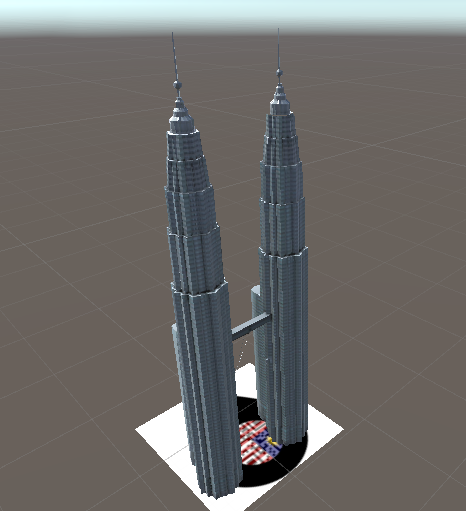
\includegraphics[width=\linewidth]{Malaysia.png}
  \caption{3D Objekt von Malaysia (Asien)}\label{fig:malaysia}
\endminipage\hfill
\end{figure}

